\chapter{SIMULATION UND TEST}
\label{sec:implementation}

Die Verifizierung ist ein sehr wichtiger Teil des Entwurfs. Um die Korrektheit des Entwurfs sicherzustellen, müssen die Simulationsergebnisse getestet und verifiziert werden.

\vspace{\baselineskip}

\noindent Tabelle 4.1 zeigt die hexadezimalen Codes, die den 27 Zuständen des endlichen Automaten des Algorithmus entsprechen, um zu überprüfen, ob im Test die richtigen Zustandsübergänge durchgeführt wurden.

\begin{table}[H]
    \caption{Hexadezimale Codierung der Zustände}
    \resizebox{\textwidth}{!}{
    \begin{tabular}{|c|c|c|c|c|c|c|c|c|c|}
      \hline
      Zustand      & IDLE      & SORT1     & SORT2     & SORT3     & SORT4     & SORT5     & SORT6     & SORT7     & SORT8     \\ \hline
      Hexcodierung & Zustand00 & Zustand01 & Zustand02 & Zustand03 & Zustand04 & Zustand05 & Zustand06 & Zustand07 & Zustand08 \\ \hline\hline
      Zustand      & SORT9     & SORT10    & SORT11    & SORT12    & SORT13    & SORT14    & SORT15    & SORT16    & SORT17    \\ \hline
      Hexcodierung & Zustand09 & Zustand0A & Zustand0B & Zustand0C & Zustand0D & Zustand0E & Zustand0F & Zustand10 & Zustand11 \\ \hline\hline
      Zustand      & SORT18    & SORT19    & SORT20    & SORT21    & SORT22    & SORT23    & SORT24    & OUTPUT1   & OUTPUT2   \\ \hline
      Hexcodierung & Zustand12 & Zustand13 & Zustand14 & Zustand15 & Zustand16 & Zustand17 & Zustand18 & Zustand19 & Zustand1A \\ \hline
    \end{tabular}}
\end{table}

\section{SIMULATION UND TEST DER FSM}

Tabelle 4.2 enthält Beispiele für drei verschiedene Eingaben und die gewünschten Ergebnisse.

\noindent Die beiden Eingabezahlen für Beispiel 1 sind 0x25 (Dezimalzahl 37) und 0x15 (Dezimalzahl 21). Sie haben keinen anderen gemeinsamen Faktor als 1, so dass ihr größter gemeinsamer Teiler 0x01 (Dezimalzahl 1) ist. Die beiden Eingabezahlen für Beispiel 2 sind 0x0F (Dezimalzahl 15) und 0x19 (Dezimalzahl 25). Sie haben andere gemeinsame Faktoren als 1, so dass ihr größter gemeinsamer Teiler 0x05 (Dezimalzahl 5) ist; die beiden Eingabezahlen für Beispiel 3 sind 0x00 (Dezimalzahl 0) und 0x06 (Dezimalzahl 6). Da die Eingabedaten 0 enthalten, wird das Ergebnis aus dem vorherigen Urteilszustand abgeleitet, d. h. ihr größter gemeinsamer Teiler ist eine andere Zahl als 0, nämlich 0x06.

\vspace{\baselineskip}

\noindent Diese Tabelle umfasst verschiedene Kombinationen von Eingabewerten. Die Tabelle ist gut geeignet, um Eingaben in verschiedenen Situationen zu testen. Die Tabelle wird verwendet, um die Korrektheit des Algorithmus zu überprüfen.

\begin{table}[H]
    \centering
    \caption{Beispiele für verschiedene Eingaben}
    \begin{tabular}{|c|c|c|c|}
      \hline
      Beispiele & MEM(0) & MEM(1) & OUTPUT \\ \hline
      1         & 0x25   & 0x15   & 0x01   \\ \hline
      2         & 0x0F   & 0x19   & 0x05   \\ \hline
      3         & 0x00   & 0x06   & 0x06   \\ \hline

    \end{tabular}
\end{table}

\noindent Wie in Abbildung 4.1 dargestellt, laufen die Eingangsdaten 0x25 und 0x15 nach der Bestimmung des Zustands in die State-Loop des euklidischen Algorithmus ein. Da der größte gemeinsame Teiler zweier Zahlen 1 ist, sind die Werte in den Registern x und y nach mehreren Zyklen (in Abbildung 4.2 sind nur die ersten vier Zyklen, LOOP1-LOOP4, bezeichnet) gleich. Dann wird die Loop beendet und das Ergebnis wird ausgegeben.

\begin{figure}[H]
    \centering
    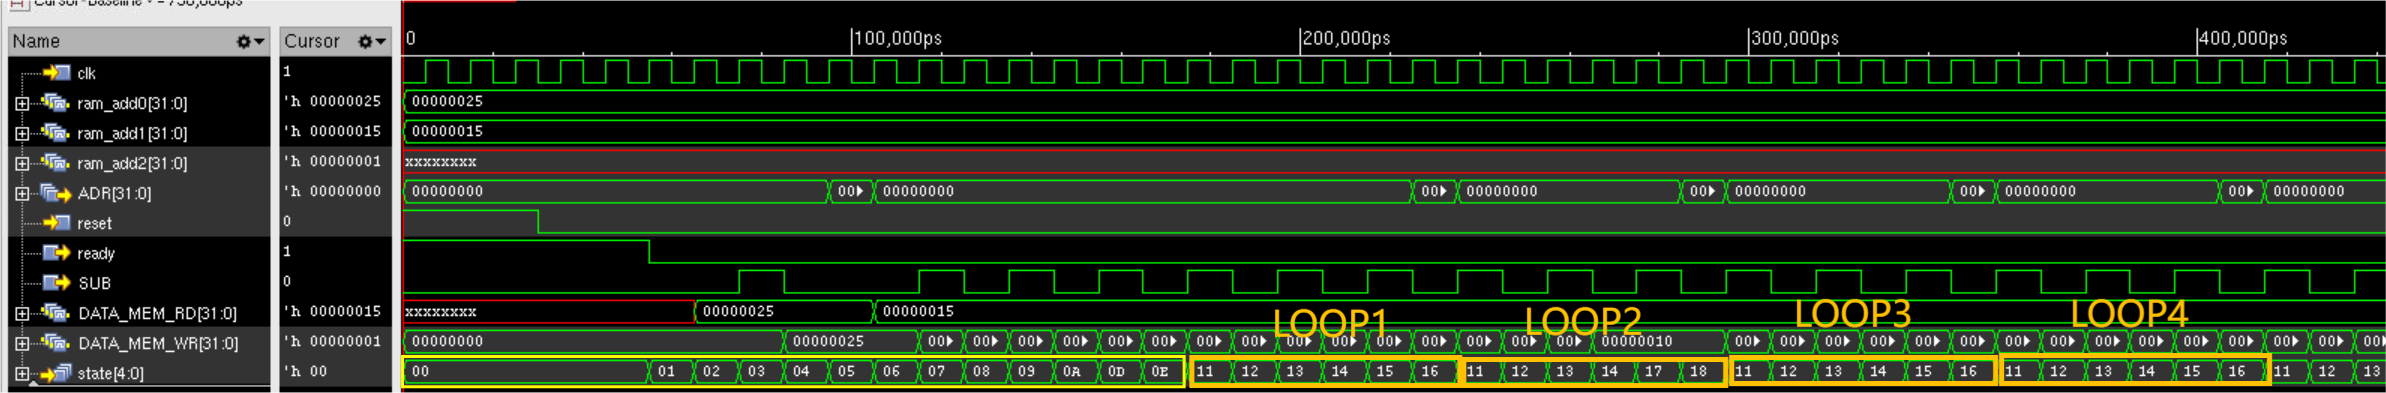
\includegraphics[width=1.0\textwidth]{images/bs1.png}
    \caption[Beispiel 1 für FSM-Simulationsergebnisse]{Beispiel 1 für FSM-Simulationsergebnisse}
    \label{fig:bs1}
\end{figure}

\noindent Beispiel 2 hat die Eingänge 0x0F und 0x19. Auch dieses Beispiel tritt nach einem Urteilszustand in die Zyklusphase des Euklidschen Algorithmus ein. Der Unterschied zwischen diesem Beispiel und Beispiel 1 besteht darin, dass der im x-Register gespeicherte Wert in diesem Beispiel kleiner ist als der im y-Register gespeicherte Wert; der im x-Register gespeicherte Wert in Beispiel 1 ist jedoch größer als der im y-Register gespeicherte Wert. Daher unterscheidet sich der Zustand von Beispiel 2 vom Zustand von Beispiel 1, als es in die Runde eintritt.

\begin{figure}[H]
    \centering
    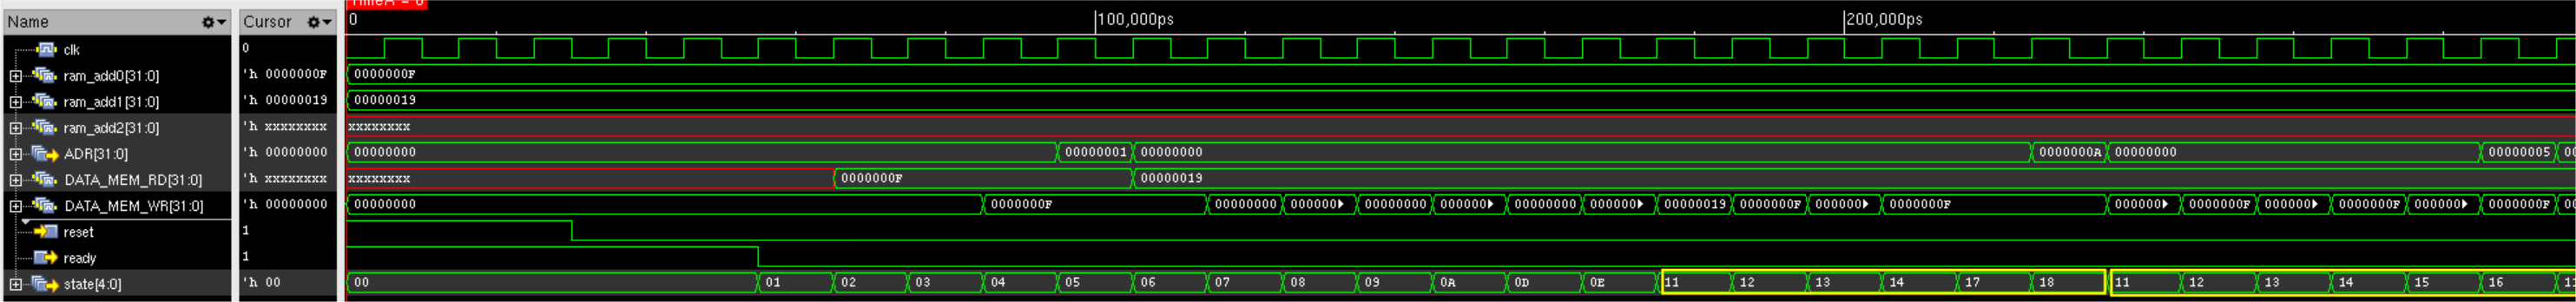
\includegraphics[width=1.0\textwidth]{images/bs2.png}
    \caption[Beispiel 2 für FSM-Simulationsergebnisse]{Beispiel 2 für FSM-Simulationsergebnisse}
    \label{fig:bs2}
\end{figure}

\noindent Der Eingang zu Beispiel 3 enthält den Wert 0x00, der die Verarbeitung der Daten und die Ausgabe des Ergebnisses in der ersten Hälfte des Urteilszustands ermöglicht.

\begin{figure}[H]
    \centering
    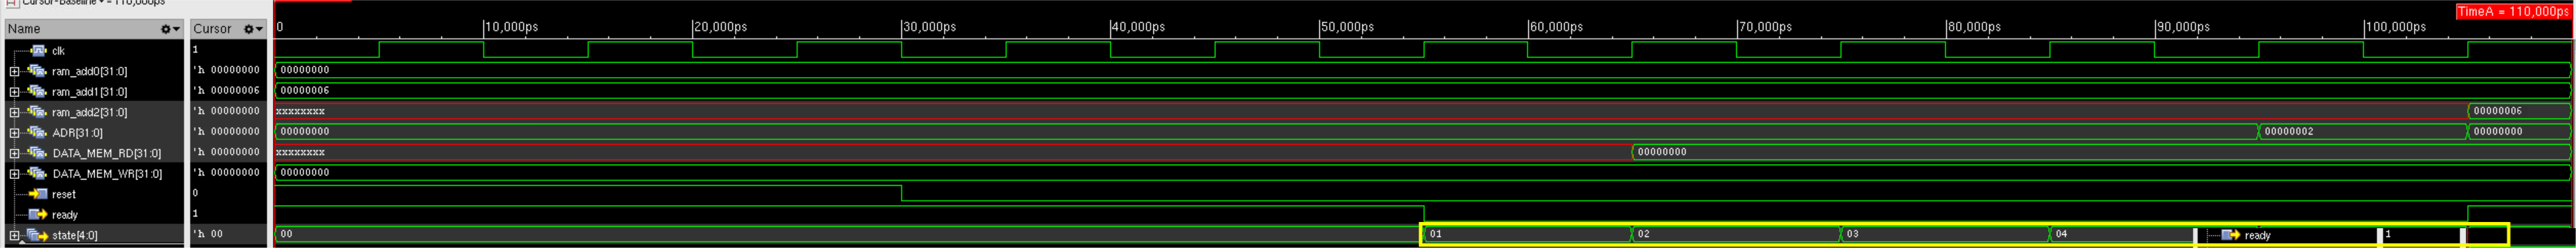
\includegraphics[width=1.0\textwidth]{images/bs3.png}
    \caption[Beispiel 3 für FSM-Simulationsergebnisse]{Beispiel 3 für FSM-Simulationsergebnisse}
    \label{fig:bs3}
\end{figure}

\section{SIMULATION UND TEST DER GESAMTSCHALTUNG}

Die Abbildungen 4.4-4.6 zeigen die Testergebnisse für die Beispiele 1-3. Die Ergebnisse der Simulationen können mit den erwarteten Ergebnissen in Tabelle 4.2 verglichen werden, um zu überprüfen, ob der Algorithmus wie erwartet funktioniert.

\begin{figure}[H]
    \centering
    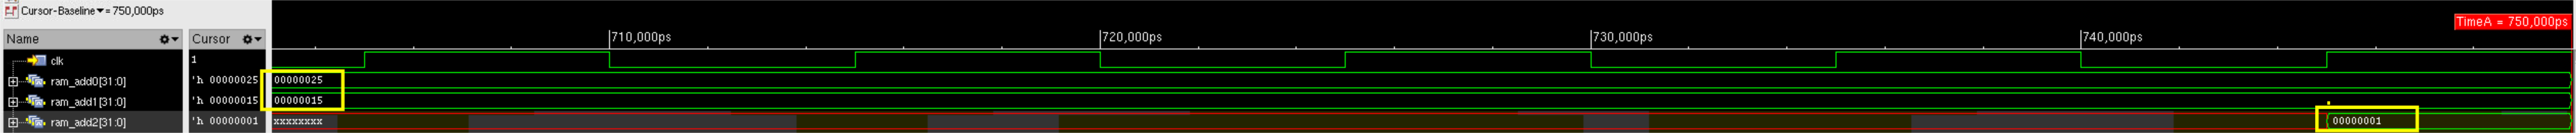
\includegraphics[width=1.0\textwidth]{images/bs1result.png}
    \caption[Beispiel1 für Simulationsergebnisse]{Beispiel1 für Simulationsergebnisse}
    \label{fig:bs1result}
\end{figure}

\begin{figure}[H]
    \centering
    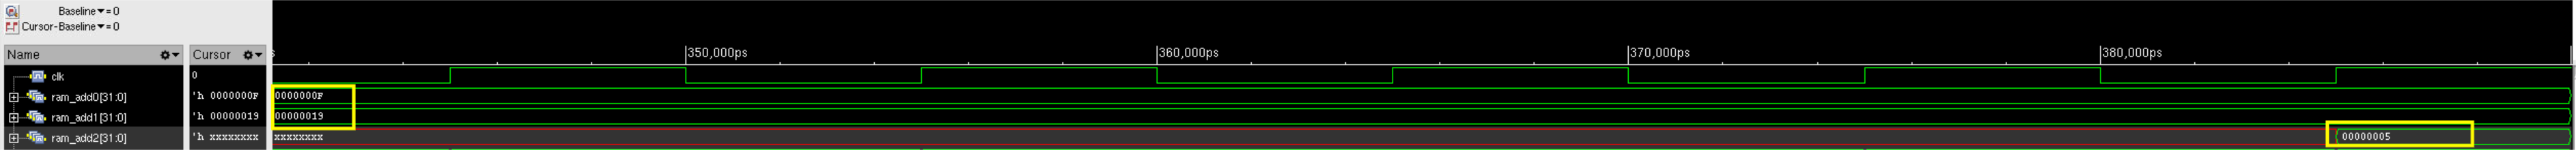
\includegraphics[width=1.0\textwidth]{images/bs2result.png}
    \caption[Beispiel2 für Simulationsergebnisse]{Beispiel2 für Simulationsergebnisse}
    \label{fig:bs2result}
\end{figure}

\begin{figure}[H]
    \centering
    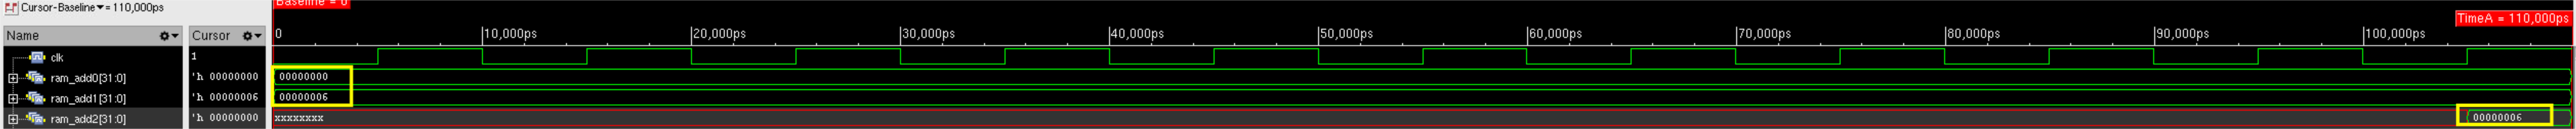
\includegraphics[width=1.0\textwidth]{images/bs3result.png}
    \caption[Beispiel3 für Simulationsergebnisse]{Beispiel3 für Simulationsergebnisse}
    \label{fig:bs3result}
\end{figure}

\noindent Es ist zu erkennen, dass die Simulationsergebnisse für alle drei Beispiele mit den erwarteten Ergebnissen des Algorithmus übereinstimmen. Dann läuft der Algorithmus korrekt.
\cleardoublepage
